%\documentclass[11pt,a4paper]{article}
\documentclass[11pt
  , a4paper
  , article
  , oneside
%  , twoside
%  , draft
]{memoir}

\usepackage{control}
\usepackage[numbers]{natbib}

\begin{document}

\newcommand{\technumber}{
  RAON Control-Document Series\\
  Revision : v0.1,   Release : Mar. 12. 2015}
\title{\textbf{EPICS와 SNMP 통합}}

\author{박미정\thanks{mijoy0909@ibs.re.kr} \\

  Rare Isotope Science Project\\
  Institute for Basic Science, Daejeon, South Korea
}
\date{\today}

\renewcommand{\maketitlehooka}{\begin{flushright}\textsf{\technumber}\end{flushright}}
%\renewcommand{\maketitlehookb}{\centering\textsf{\subtitle}}
%\renewcommand{\maketitlehookc}{C}
%\renewcommand{\maketitlehookd}{D}

\maketitle

\begin{abstract}
본 문서는 중이온 가속기 제어의 기본 Framework이 되는 EPICS와 SNMP통합에 관한 문서이다. 가속기 제어 시스템에 사용되는 다양한 장비를 모니터링 및 제어하는 EPICS와 SNMP 통합 모니터링 시스템의 구현에 대해 논한다.
\end{abstract}

\chapter{EPICS와 SNMP의 통합}
EPICS(Experimental Physics and Industrial Control System)는 Los Alamos국립 연구소와, Argonne국립 연구소에서 공동개발 되었으며, 오픈 라이센스로 제공된다. 입자가속기, 천체망원경 그리고 거대과학실험에서 사용되는 실시간 분산 제어 시스템인 EPICS는 현재 전 세계의 과학시설의 개발자들에 의해 개발이 진행되고있다. EPICS는 중이온 가속기 제어의 기본 Framework으로 EPICS와 SNMP의 통합은 중이온 가속기 중앙 제어 시스템의 일관성, 유지관리의 용이성, 그리고 최적화 기술의 습득 및 축적의 관점에서 중요하다. 

\section{EPICS란?}
EPICS는 실시간 분산 제어 시스템이며, 네트워크로 연결된 다양한 장비들의 모니터링 및 제어를 위해 사용된다. EPICS는 그림 \ref{fig:ca})의 EPICS 로고와 같이 네트워크 기반의 클라이언트/서버 구조이며, IOC(Input Output Controllers)를 통해 동작한다. 클라이언트와 서버는 CA(Channel Access)라는 통신 프로토콜을 사용하여 PV(Process Variable)라는 데이터를 주고 받는다. CA클라이언트는 PV를 요청하며, CA서버는 가능한 PV를 제공한다.  CA는 특히 높은 대역폭, 소프트 실시간 네트워크로 제어가 요구되는 응용프로그램들에 맞춰 설계되었고, 이는 엄청난 수의 컴퓨터와 장비들을 포함한 제어시스템 구축에 EPICS가 사용될 수 있는 이유이다. 또한 EPICS는 신뢰성을 제공하며, 이미 구축된 시스템의 유지보수가 용이하다는 장점이 있다. 

\begin{figure}[h!]
  \centering
  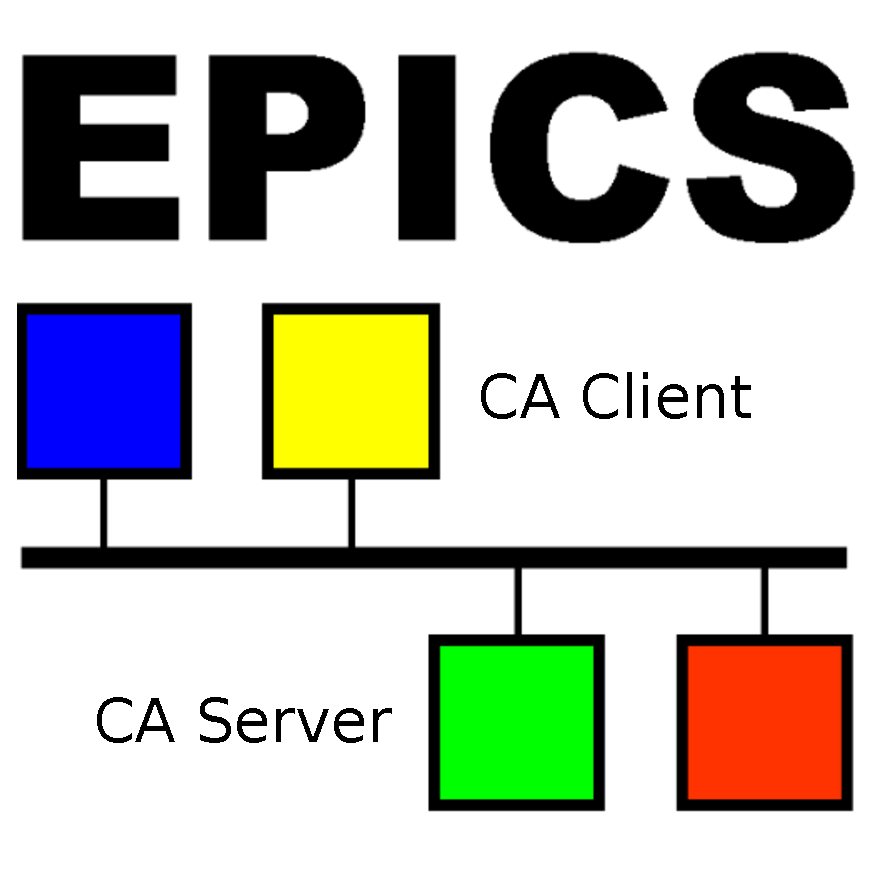
\includegraphics[width=0.3\textwidth]{./images/epics.eps}
  \caption{Channel Access 구조}
  \label{fig:ca}   
\end{figure}

\section{SNMP란?}
SNMP(Simple Network Management Protocol)\footnote{* SNMP에 관한 자세한 설명은 SNMP 이해 및 응답시간 테스트를 참조 바란다.}는 IP네트워크 상의 장치 및 장비들을 관리하고 모니터링하기 위한 인터넷 표준 프로토콜이다. SNMP는 인증과 암호화에 따른 차이점으로 v1/2c/3 세 가지로 나뉘며, 그림\ref{fig:relationship_m_a}와 같이 Manager와 Agent로 구성되어있다. Manager는 Agent에게 원하는 장비의 정보를 요청하며, 장비의 설정을 변경한다. Agent는 Manager가 요청한 장비의 정보를 제공하고, 시스템 충돌이나 재부팅 등의 장비에 영향을 미치거나 발생한 Event를 비동기적으로 알리기 위해 Trap 메세지를 보낸다. 장비의 정보들은 OID(Object Identifiers)객체라 하며, MIB(Management Information Base)내에 계층구조를 이룬다. 일반적인 TCP/IP관리정보는 MIB-2(RFC 1213)에 포함돼있고, 특정 장비들의 정보는 장비제조업체에서 제공한다. 

\begin{figure}[h!]
  \centering
  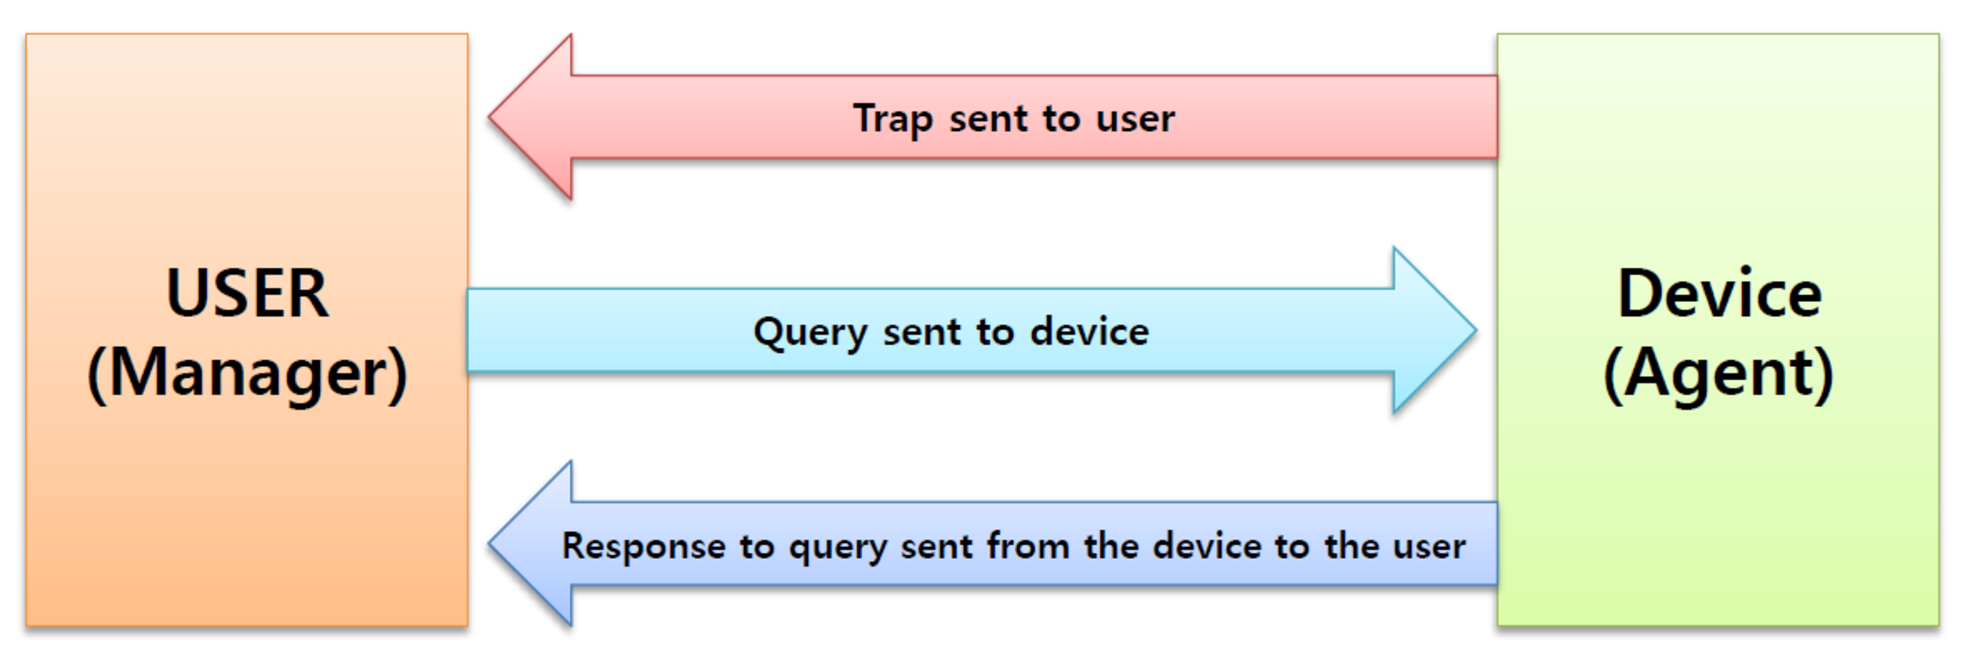
\includegraphics[width=0.65\textwidth]{./images/relationship_m_a.eps}
  \caption{Manager와 Agent의 관계}
  \label{fig:relationship_m_a}   
\end{figure}



\chapter{SNMP Device Support Moudle}

SNMP의 MIB는 EPICS에서 PV(Process Variable)과 동일하다. 

SNMP로 모니터링 및 제어 할 장비에 맞춰 Labrary와 DB파일 등의 EPICS IOC(Input-Output Controller)를 개발하고, CA(Channel Access)를 통한 통신을 목적으로 한다. 





\section{FRIB SNMP Device Support Moudle}
\subsection{subsection}

\section{Figure and Itemize}
 Figure shows the vmplayer screen-shot of the MAC address for a virtual PC.

For the installation examples, two MAC addresses and the hostnames are used as follows :
\begin{itemize}
\item demohost  : \texttt{E8:03:9A:63:83:81}
\\item gnomehost : \texttt{00:50:56:39:D9:1E}
\end{itemize}



\clearpage

\chapter{Legacy SNMP Code}
\section{Net-snmp tutorial}

\begin{itemize}
  \item \texttt{/etc/fai}
    {\scriptsize
     \begin{verbatim}
      root@faiserver:/etc/fai# tree
      .
      ├── apt
      │   └── sources.list
      ├── fai.conf
      ├── grub.cfg
      ├── live.conf
      ├── NFSROOT
      └── nfsroot.conf
     \end{verbatim}
     }
  \item \texttt{/srv/fai}
    {\scriptsize
     \begin{verbatim}
      root@faiserver:/srv# tree -d -L 3
      .
      ├── fai
      │   ├── config
      │   │   ├── basefiles
      │   │   ├── class
      │   │   ├── debconf
      │   │   ├── disk_config
      │   │   ├── files
      │       ├── selinux
      │       ├── srv
      │       ├── sys
      │       ├── tmp
      │       ├── usr
      │       └── var
      └── tftp
            └── fai
                  └── pxelinux.cfg
  \end{verbatim}
  }
\end{itemize}

\subsection{lstlisting with termstyle}


\clearpage
\bibliographystyle{unsrtnat}
\bibliography{./refs}

\end{document}
